\documentclass[fleqn]{article}
\usepackage[margin=1in]{geometry}
\usepackage[nodisplayskipstretch]{setspace}
\usepackage{amsmath, nccmath, bm}
\usepackage{amssymb}
\usepackage{enumitem}
\usepackage{graphicx}
\usepackage{float}
\usepackage{listings}
\usepackage{hyperref}
\usepackage[svgnames]{xcolor}
\graphicspath{{./images}}

\hypersetup{
    colorlinks=true,
    linkcolor=black,
    filecolor=black,      
    urlcolor=blue
    }

\newcommand{\zerodisplayskip}{
	\setlength{\abovedisplayskip}{0pt}%
	\setlength{\belowdisplayskip}{0pt}%
	\setlength{\abovedisplayshortskip}{0pt}%
	\setlength{\belowdisplayshortskip}{0pt}%
	\setlength{\mathindent}{0pt}}
	
\definecolor{vgreen}{RGB}{104,180,104}
\definecolor{vblue}{RGB}{49,49,255}
\definecolor{vorange}{RGB}{255,143,102}

\lstdefinestyle{verilog-style}
{
    language=Verilog,
    basicstyle=\small\ttfamily,
    keywordstyle=\color{vblue},
    identifierstyle=\color{black},
    commentstyle=\color{vgreen},
    numbers=left,
    numberstyle=\tiny\color{black},
    numbersep=10pt,
    tabsize=8,
    moredelim=*[s][\colorIndex]{[}{]},
    literate=*{:}{:}1
}

\lstset{style={verilog-style},showstringspaces=false}

\makeatletter
\newcommand*\@lbracket{[}
\newcommand*\@rbracket{]}
\newcommand*\@colon{:}
\newcommand*\colorIndex{%
    \edef\@temp{\the\lst@token}%
    \ifx\@temp\@lbracket \color{black}%
    \else\ifx\@temp\@rbracket \color{black}%
    \else\ifx\@temp\@colon \color{black}%
    \else \color{vorange}%
    \fi\fi\fi
}
\makeatother

\newcommand{\code}[1]{%
	\colorbox{Gainsboro}{\texttt{#1}}%
}

\title{Lab 1}
\author{Owen Sowatzke}
\date{March 17, 2025}

\begin{document}

	\offinterlineskip
	\setlength{\lineskip}{12pt}
	\zerodisplayskip
	\maketitle
	
	\section{Introduction}
	
	\section{Procedure}
	
	\section{Results}
	
	\subsection{First Order Transistor Model}
	
	\texttt{let ids=-vds\#branch}
	
	\texttt{let ids\_p=deriv(ids)}
	
	\texttt{plot ids\_p}
	
	\texttt{let ids\_pp=deriv(ids\_p)}
	
	\texttt{meas dc m max ids\_pp}
	
	\texttt{meas dc vgs\_i max\_at ids\_pp}
	
	\texttt{meas dc ids\_p\_i find ids\_p when vgs=vgs\_i}
	
	\texttt{let b = ids\_p\_i - m*vgs\_i}
	
	\texttt{let vt = -b/m}
	
	\texttt{print vt}
	
	\texttt{let ids\_p\_fit = m*vgs + b}
	
	\texttt{plot ids\_p ids\_p\_fit yrange}
	
	\begin{center}
	\begin{tabular}{| c | c |}
		\hline
		Parameter & Value \\
		\hline	
		$V_{t0}$ & $0.6613 V$\\
		\hline	
		$V_{dsat}$ & $0.3948 V$\\
		\hline	
		$\lambda$ & $0.1289 V^{-1}$\\
		\hline			
		$k_n$ & $164.1 {\mu}A/V^2$ \\
		\hline
	\end{tabular}
	\end{center}
	
	\subsection{NAND Gate}
	
	\subsubsection{Design}
	
	The pull-down circuit of the NAND gate is composed of two sequential NMOS gates. The pull-up circuit is the complement and is composed of two parallel PMOS gates. Note that we also increase the width of the PMOS transistor by a factor of 2 to account for the lower mobility of holes in the p-type material. The schematic for the resulting circuit is shown in Figure \ref{fig::nand_schematic}.
	
	\begin{figure}[H]
		\centerline{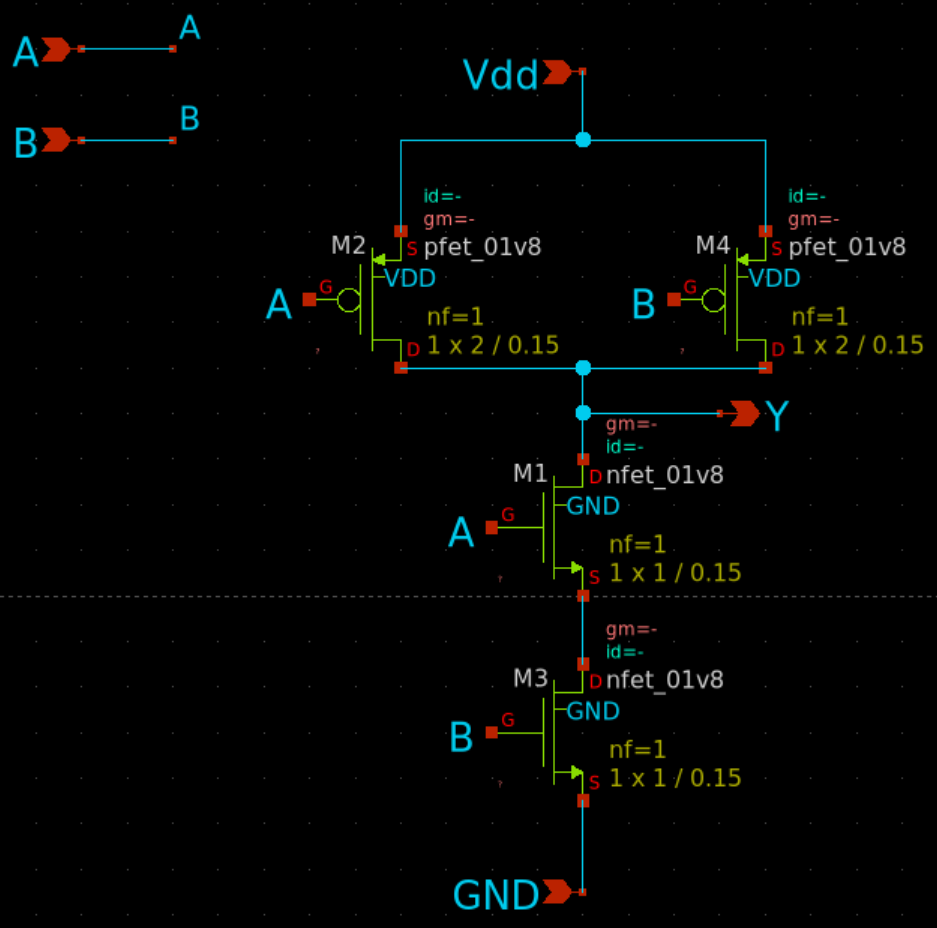
\includegraphics[width=0.4\textwidth]{nand_schematic.png}}
		\caption{NAND Circuit Schematic}
		\label{fig::nand_schematic}
	\end{figure}

	We also create a circuit symbol for the NAND gate, which is shown in Figure \ref{fig::nand_symbol}.
	
	\begin{figure}[H]
		\centerline{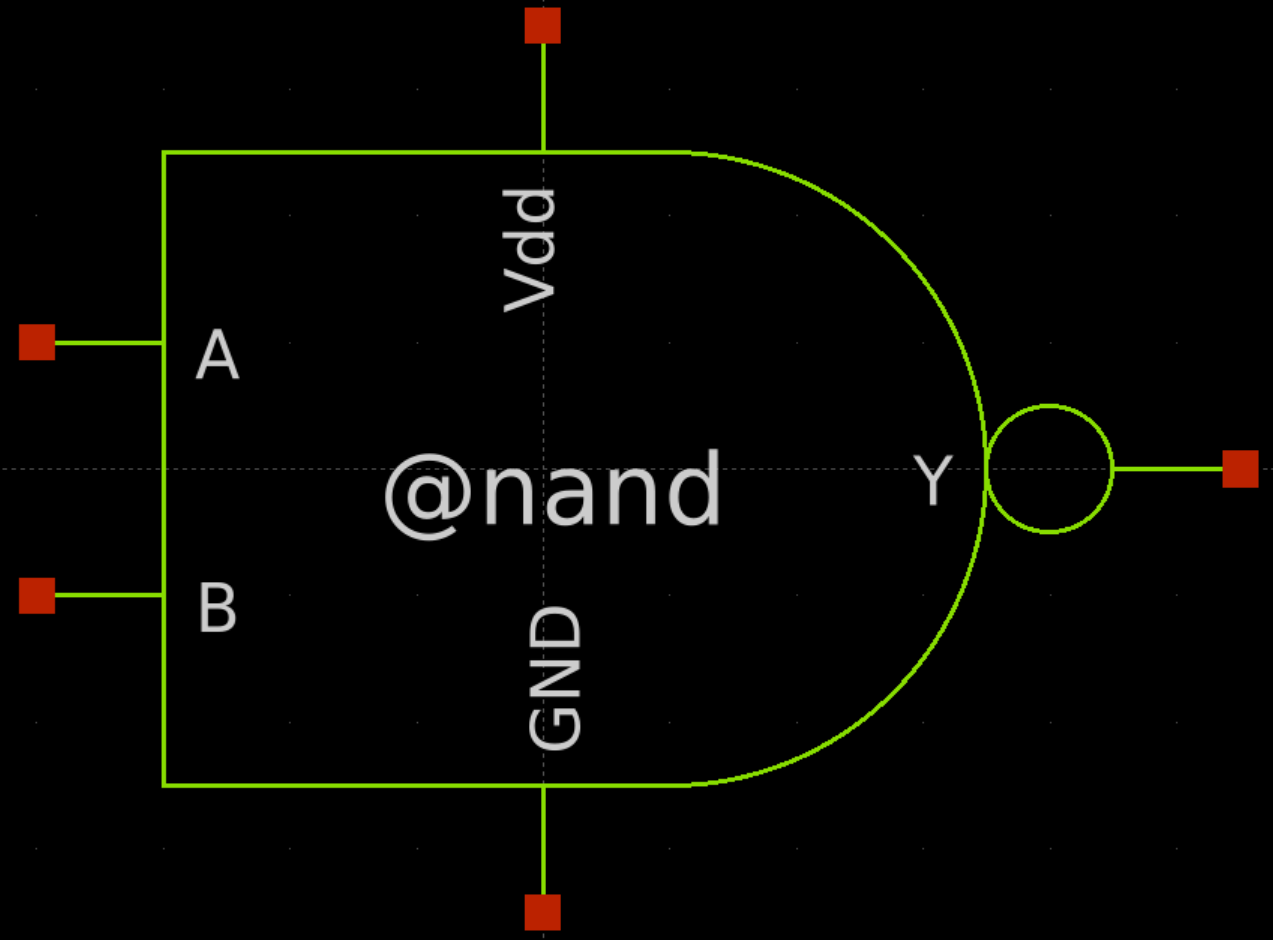
\includegraphics[width=0.4\textwidth]{nand_symbol.png}}
		\caption{NAND Circuit Symbol}
		\label{fig::nand_symbol}
	\end{figure}
	
	\subsubsection{Voltage Transfer Characteristics}
	
	In this section, we analyze the voltage transfer characteristics (VTC) of our NAND gate. For this analysis, we analyze the VTC when varying \texttt{a} and \texttt{b} independently and when varying \texttt{a} and \texttt{b} together. The test circuit we use when just varying the input \texttt{a} is included in Figure \ref{fig::nand_vtc_test_sweep_va}.
	
	\begin{figure}[H]
		\centerline{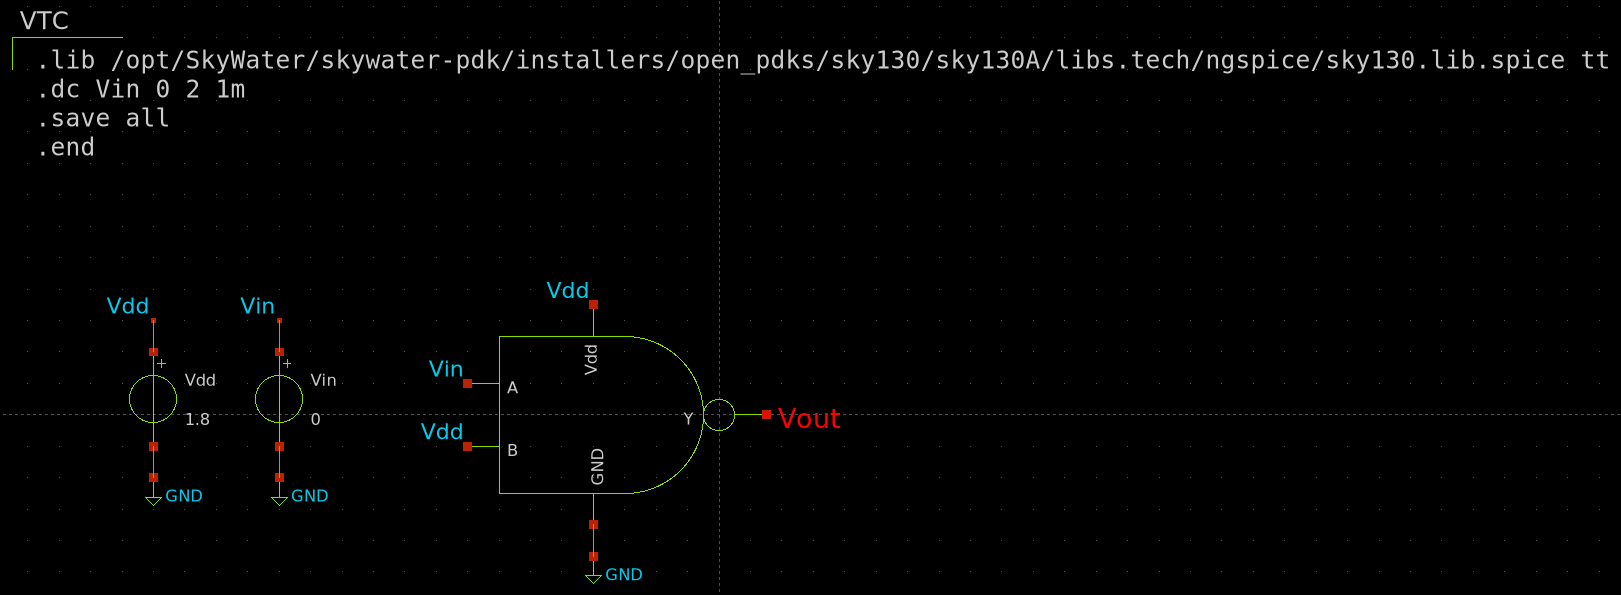
\includegraphics[width=0.8\textwidth]{nand_vtc_test_sweep_va.png}}
		\caption{NAND VTC Test Circuit for Independent Variations of Input \texttt{a}}
		\label{fig::nand_vtc_test_sweep_va}
	\end{figure}
	
	Using this test circuit, we perform DC analysis to determine the VTC and find \texttt{Va}, which is the voltage at which \texttt{Vin = Vout}. The results of this analysis are shown in Figure \ref{fig::nand_vtc_sweep_va}.
	
	\begin{figure}[H]
		\centerline{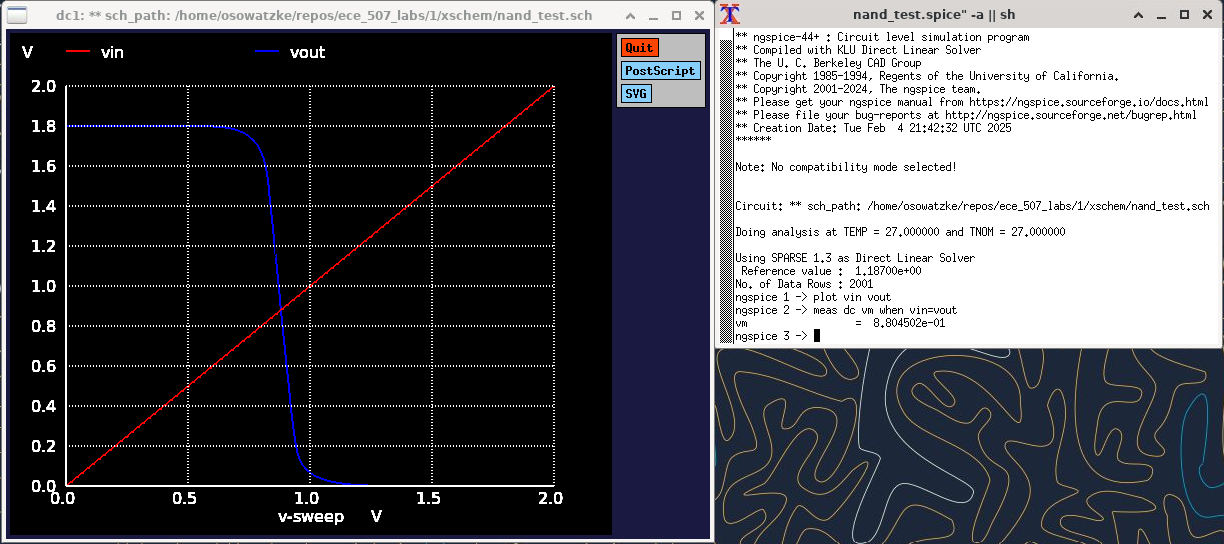
\includegraphics[width=0.8\textwidth]{nand_vtc_sweep_va.png}}
		\caption{NAND VTC Results for Independent Variations of Input \texttt{a}}
		\label{fig::nand_vtc_sweep_va}
	\end{figure}
	
	Examining the results, we find that \texttt{Vm = 0.8805V}. We perform similar analysis for independent variations of the input \texttt{b}. The test circuit and results are attached in figures \ref{fig::nand_vtc_test_sweep_vb} and \ref{fig::nand_vtc_sweep_vb} independently.
	
	\begin{figure}[H]
		\centerline{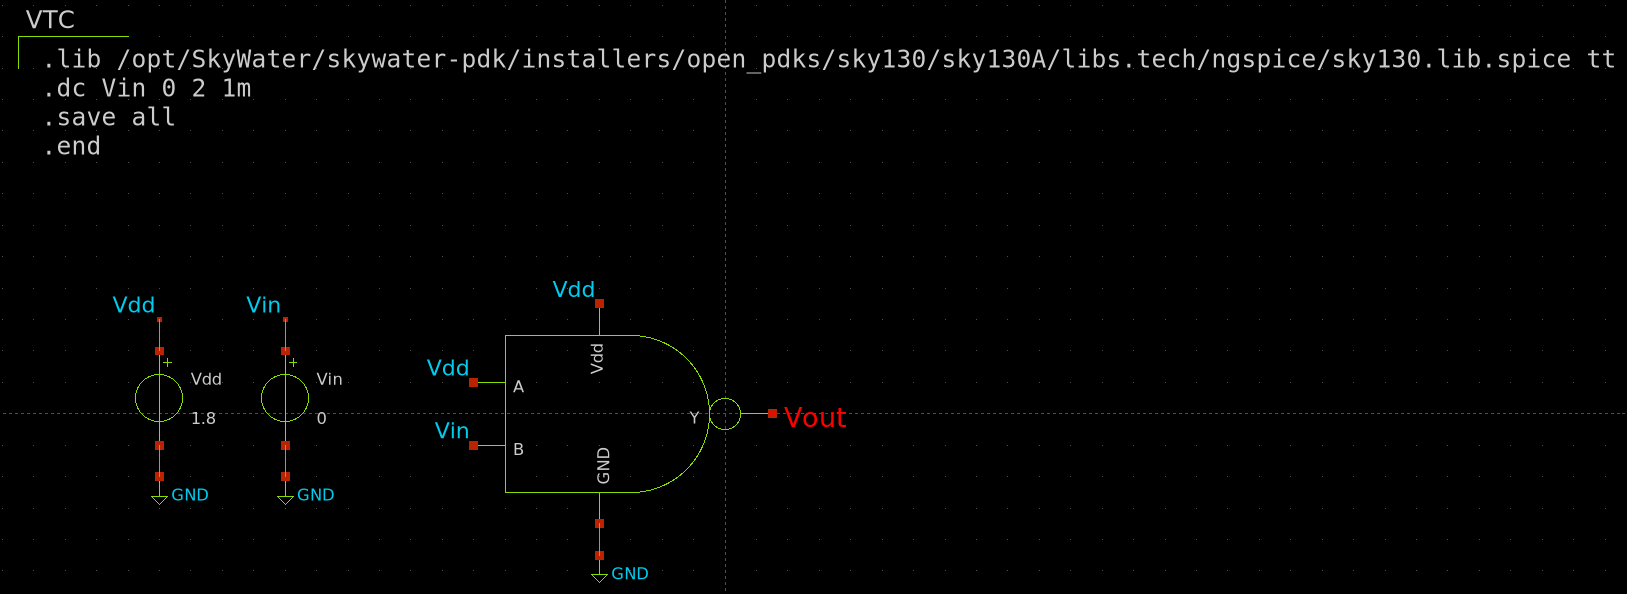
\includegraphics[width=0.8\textwidth]{nand_vtc_test_sweep_vb.png}}
		\caption{NAND VTC Test Circuit for Independent Variations of Input \texttt{b}}
		\label{fig::nand_vtc_test_sweep_vb}
	\end{figure}
	
	\begin{figure}[H]
		\centerline{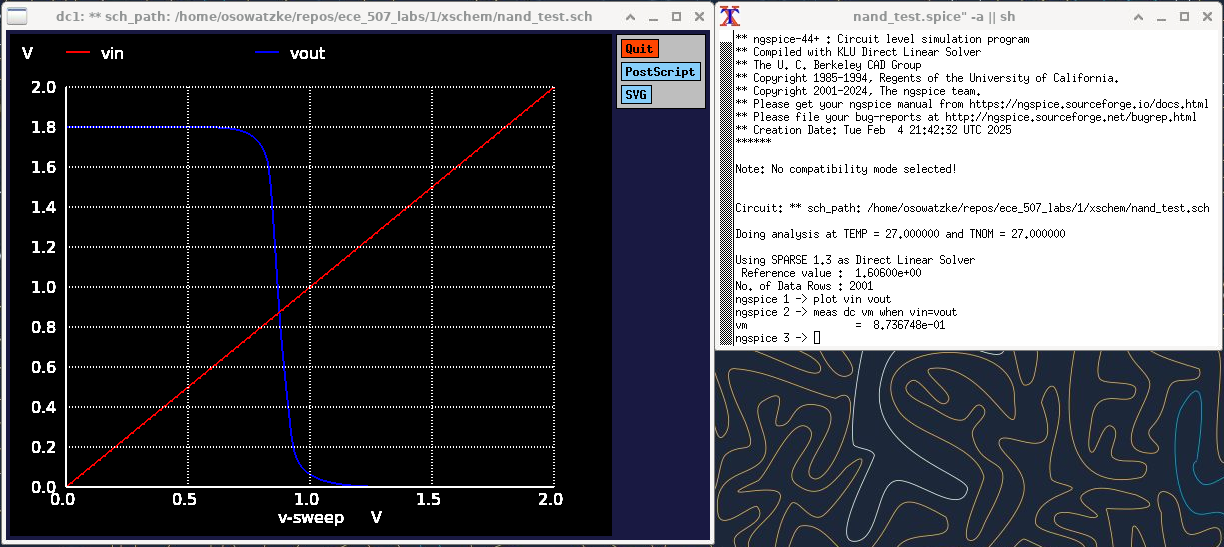
\includegraphics[width=0.8\textwidth]{nand_vtc_sweep_vb.png}}
		\caption{NAND VTC Results for Independent Variations of Input \texttt{b}}
		\label{fig::nand_vtc_sweep_vb}
	\end{figure}
	
	Examining the results, we find that \texttt{Vm = 0.8737V}. Finally, we sweep both inputs \texttt{a} and \texttt{b} together. The test circuit and results for this analysis are included in Figures \ref{fig::nand_vtc_test_sweep_va_vb} and \ref{fig::nand_vtc_sweep_va_vb} respectively.
	
	\begin{figure}[H]
		\centerline{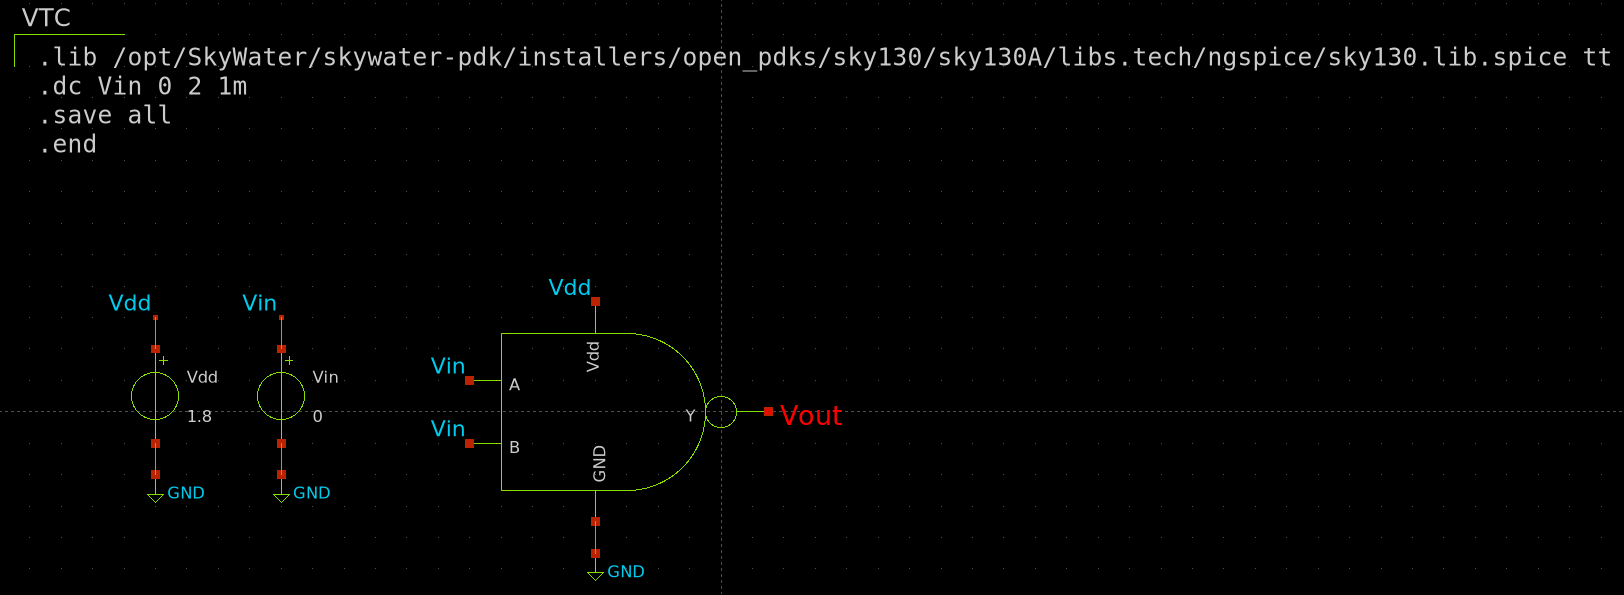
\includegraphics[width=0.8\textwidth]{nand_vtc_test_sweep_va_vb.png}}
		\caption{NAND VTC Test Circuit for Joint Variations of Inputs \texttt{a} and \texttt{b}}
		\label{fig::nand_vtc_test_sweep_va_vb}
	\end{figure}
	
	\begin{figure}[H]
		\centerline{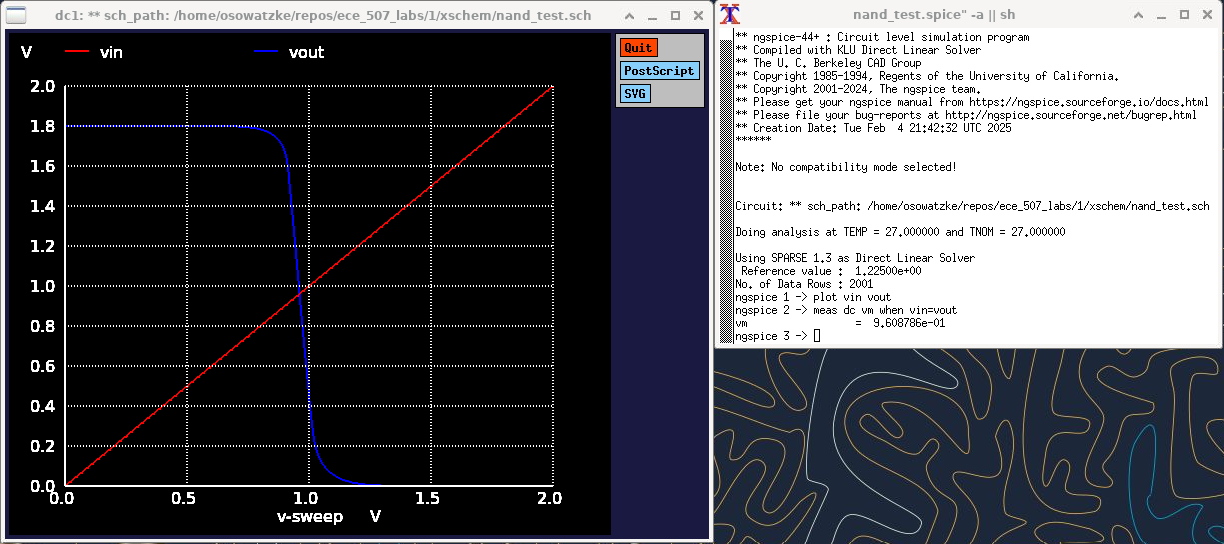
\includegraphics[width=0.8\textwidth]{nand_vtc_sweep_va_vb.png}}
		\caption{NAND VTC Results for Joint Variations of Inputs \texttt{a} and \texttt{b}}
		\label{fig::nand_vtc_sweep_va_vb}
	\end{figure}
	
	Examining the results, we find that \texttt{Vm = 0.9609V}.
	
	\begin{figure}[H]
		\centerline{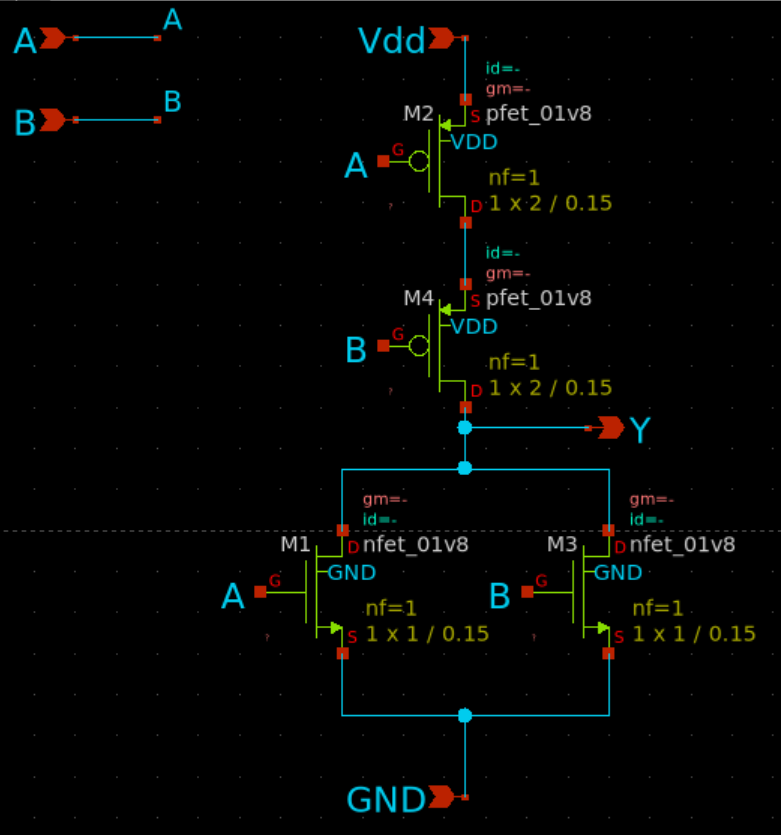
\includegraphics[width=0.4\textwidth]{nor_schematic.png}}
		\caption{NOR Circuit Schematic}
		\label{fig::nor_schematic}
	\end{figure}
	
	\begin{figure}[H]
		\centerline{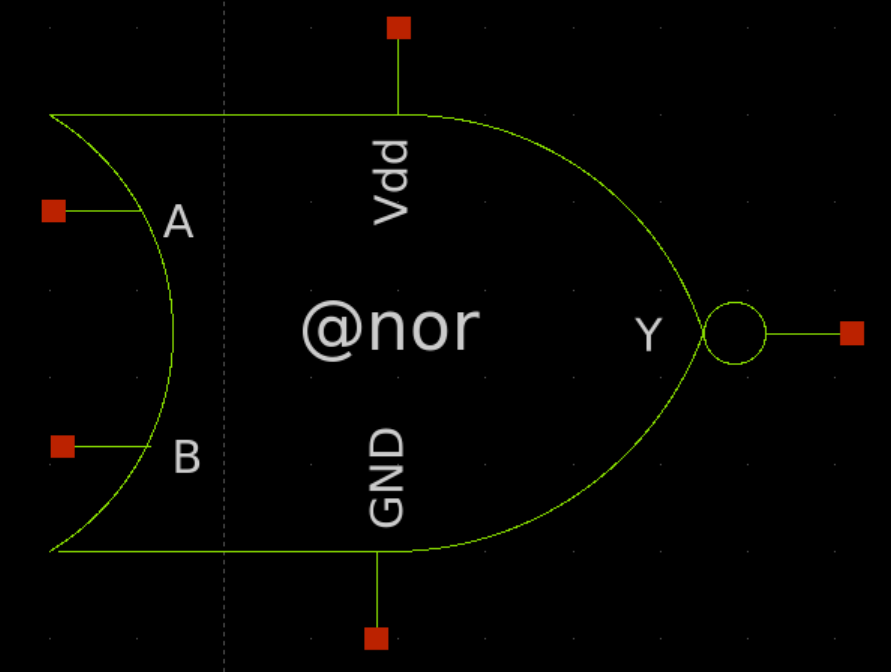
\includegraphics[width=0.4\textwidth]{nor_symbol.png}}
		\caption{NOR Circuit Symbol}
		\label{fig::nor_symbol}
	\end{figure}
	
	\subsection{NAND Gate}

\end{document}